This chapter presents background information on virtualization and confinement
technologies in Linux and other Unix-like operating systems. It also presents a detailed
history and examination of \gls{ebpf} and discusses its applications in the domains of computer
security, performance monitoring, and beyond.

\section{Process-Level Virtualization and Confinement}%
\label{s:virtualization-and-confinement}

Unlike virtual machines, containers are nothing but a collection of related processes
(sometimes just one process, but often more) running on the host operating system. These
processes share the same kernel as other running containers and as \enquote{native}
processes running outside of a container. While these properties can help containers to be
lighter-weight than virtual machines, they also necessitate the usage of process-level
virtualization and confinement primitives to isolate containers from one
another~\cite{sultan2019_container_security}.  \Cref{s:container-security-bg} covers
containers and container security in greater detail, further differentiating them from
VMs. For the purposes of this section, it is enough to know that containerized processes
run directly on the host, share the host kernel, and use virtualization and confinement
primitives to achieve isolation.

While containers rely on virtualization and confinement primitives to facilitate normal
operation, this notion of process isolation predates the advent of containers by decades.
Isolation of processes, particularly in the case of multi-tenant and network-facing
systems, makes a lot of sense from the persecutive of security best-practices. Locking
down a program such that it can only perform the actions required for it to function
correctly can help reduce attack surface and minimize the potential for damage to the rest
of the system in the event of compromise. This notion of restricting a program's
capabilities to the minimal viable set has a name in the security literature: the
\textit{principle of least-privilege}~\cite{schneider03_least_privilege,
van_oorschot2020_tools_jewels}.

Researchers have been studying confinement for decades~\cite{lampson1973_confinement}, and
have been designing and applying confinement primitives since the early days of
time-sharing computers and multi-tenant systems~\cite{shu2016_security_isolation_study}.
Process-level virtualization has become similarly important, but for subtly different
reasons\,---\,namely, for the purpose of restricting and modifying a process' visibility
into the rest of the system.  Decades of research into virtualization and confinement
techniques has culminated in a wealth of knowledge and prior artifacts, some of which have
seen widespread deployment and remain relevant to date. The rest of this section presents
technical background on such process-level virtualization confinement mechanisms and
surveys the academic literature related to this area.

\subsection{Virtual Memory and Memory Protection}%
\label{ss:virtual-memory}

\subsubsection*{CPU Protection Rings}

\begin{inprogress}
  \begin{itemize}
    \item Multics protection rings
    \item Adoption of protection rings by modern CPUs (simplified model, rings 0-3)
    \item CPU supports rings lower than 0 (really just virtualizing ring 0) for the hypervisor, CPU engine
    \item Userspace, kernelspace
  \end{itemize}
\end{inprogress}

\subsubsection*{Virtual Memory}

\begin{inprogress}
  \begin{itemize}
    \item Page tables, page table walk
    \item CPU's MMU, maps virtual addresses to physical addresses
    \item Shared memory
    \item Memory protection bits
    \item ASLR, KASLR
  \end{itemize}
\end{inprogress}

\subsection{The Reference Monitor}%
\label{ss:refmon}

The \textit{reference monitor concept}, first introduced in the landmark 1972 Anderson
Report~\cite{anderson1972_report}, was among the earliest complete descriptions of a full
access control mechanism and remains influential in operating system design to date. The
reference monitor is an abstract model for a secure reference validation mechanism built
into the operating system. The model partitions the system into \textit{subjects} (users,
processes, etc.) and \textit{objects} (system resources).  Subjects request access to
objects and the reference monitor checks this access against a known list of allowed
accesses, parameterized by the subject, object, and requested access. The software
implementation of a reference monitor is known as the \textit{security kernel.}
\Cref{fig:refmon} depicts the reference monitor concept as it was first presented by
Anderson~\cite{anderson1972_report}.

\begin{figure}[tbp]
  \centering
  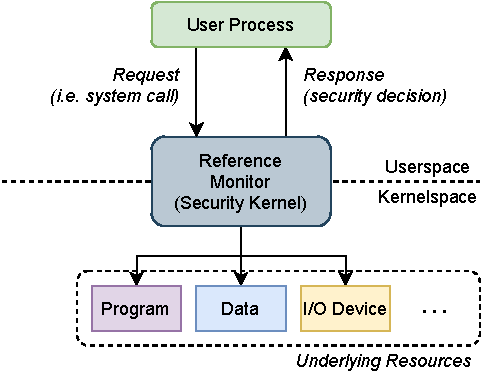
\includegraphics[width=0.6\linewidth]{figs/background/refmon.pdf}
  \caption[The reference monitor concept]{
    The reference monitor concept as outlined in the Anderson
    Report~\cite{anderson1972_report}. User processes make requests (e.g.~via system calls
    to the operating system). The \gls{os} kernel invokes the reference monitory, which is
    implemented in software as a security kernel. The reference monitor queries its
    security policy taking the subject, object, and other parameters as input. As output,
    it returns a security decision (i.e.~whether the requested access should be
    \textit{allowed} or \textit{denied}).
  }%
  \label{fig:refmon}
\end{figure}

While the majority of modern operating systems do not include a security kernel as
described by Anderson, the reference monitor architecture has informed the design of
modern access control mechanisms and models the reference validation process that occurs
when the kernel is servicing userspace requests (i.e.~system
calls)~\cite{van_oorschot2020_tools_jewels}. In order for such a design to be considered
valid, Anderson enumerate three key properties: (i) Tamper Resistance; (ii) Complete
Mediation; and (iii) Verifiability. These properties can inform the way we reason about
and design modern access control mechanisms, even if they do not strictly adhere to the
reference monitor model.

\paragraph*{Tamper-Resistance}

In order for the reference monitor to be considered \textit{tamper-resistant}, an unauthorized
party must not be able to alter the reference monitor's code or modify any data
(e.g.~memory, persistent storage) that the reference monitor relies on to enforce correct
reference validation~\cite{anderson1972_report}. This property follows from the fact that
unauthorized tampering with the reference monitor totally invalidates any security
guarantees.

\paragraph*{Complete Mediation}

The property of \textit{complete mediation} means that the reference monitor should be
invoked on all security sensitive events. It should be impossible for an attacker to
bypass the reference monitor in any way. Any software that is not subject to reference
validation should be considered a part of the reference
monitor~\cite{anderson1972_report}.

\paragraph*{Verifiability}

\textit{Verifiability} refers to the ability to reason about or prove the correctness of
the reference monitor (i.e. that the first two properties hold). Formal verification methods
are the best way of achieving verifiability, although this may not necessarily be practical
for highly complex systems. For this reason, it is recommended to design the reference monitor
in such a way that verifiability is maximized~\cite{anderson1972_report}.

\subsection{Discretionary Access Control}%
\label{ss:dac}

\textit{Discretionary access control} (DAC) forms the most basic form of access control in
many operating systems, including Linux and other Unix-like operating systems, and
Microsoft Windows. First formalized in the 1983 US Department of Defense (sic)
standard~\cite{orange_book}, a discretionary access control mechanism partitions and
labels system objects (i.e.~resources such as files) by the subjects (i.e.~actors such as
users and user processes) that \textit{own} them. The corresponding resource owner then
has full authority to decide which subjects have access to its owned objects. This notion
of ultimate authority over a subject's owned objects constitutes the primary difference
between discretionary access control and mandatory access control, which is covered in
\Cref{ss:mac}.

Classically, Unix-like systems have implemented discretionary access control in the form
of \textit{permission bits} and \textit{access control lists}. Each process on the system
runs under a specific user and group ID, which uniquely identify the user and group of the
process respectively, where each group is a collection of one or more users. Permission
bits and access control lists denote access permissions according to the user ID and group
ID of the process requesting the resource. These permissions can in turn be overridden by
the \textit{superuser} or \textit{root}~\cite{van_oorschot2020_tools_jewels,
jaeger2008_os_security}.

\subsubsection*{Permission Bits}

Permission bits in Unix are special metadata associated with a file that determine
coarse-grained access to the file according to a subject's \gls{uid} and \gls{gid}.
Permission bits are divided into three sections: \textit{User}, \textit{Group}, and
\textit{Other}. The \textit{User} bits apply to subjects whose \gls{uid} matches the
resource owner's \gls{uid}, while the \textit{Group} bits consider the \gls{gid} instead.
In all other cases (i.e.~when neither the \gls{uid} nor the \gls{gid} matches), the
\textit{Other} bits determine the allowed access. To determine which access should be
allowed, permission bits encode a coarse-grained \textit{access vector}, specifying read,
write, and execute access on a file or directory (in the case of a directory, execute
access implies the ability to \texttt{chdir(2)} into that directory).

While convenient, permission bits are generally insufficient to provide legitimate
security guarantees to modern systems~\cite{van_oorschot2020_tools_jewels,
jaeger2008_os_security}. In particular, permission bits encode coarse-grained permissions
and apply these permissions in a coarse-grained, all-or-nothing, manner. For instance,
consider the use case of granting read-only access to another user. Specifying such access
as part of the \textit{Other} bitmask implies granting access to any user on the system.
Specifying access to a particular \textit{Group} is slightly better, but the resource
owner has no direct control over which other users belong to this group, now or in the
future. Thus, we cannot say with certainty that we may specify such access without
violating our security assumptions.

\subsubsection*{Access Control Lists}

\Glspl{acl} offer a slightly more granular alternative to permission bits,
at the expense of increased complexity~\cite{jaeger2008_os_security,
van_oorschot2020_tools_jewels}. Unlike permission bits, which rely on three coarse-grained
subject categories (\textit{User}, \textit{Group}, and \textit{Other}), an access control
list defines a set of subjects and their corresponding permissions for every object. It
may be helpful to think of this as breaking up the \textit{Other} category into distinct
subjects rather than granting or revoking blanket access to all other users on the system.

Capability lists, complementary to access control lists, define a set of objects and
allowed access patterns for every subject. A capability list for a given subject can be
derived by taking the set of all access control lists for every object and vice
versa~\cite{van_oorschot2020_tools_jewels}. Together, the set of all access control lists
(or capability lists) forms an \textit{access matrix}, describing the \gls{dac} policy over
the entire system. \Cref{fig:acl} depicts this relationship.

\begin{figure}[tbp]
  \centering
  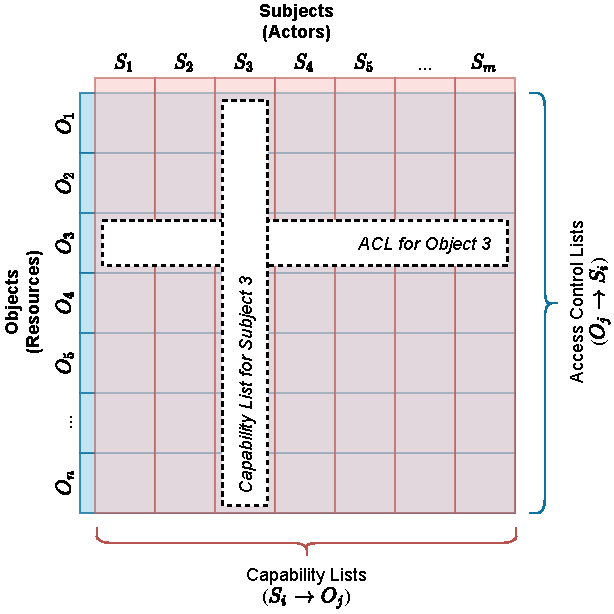
\includegraphics[width=0.8\linewidth]{figs/background/acl.pdf}
  \caption[The access matrix]{
    The access matrix and the relationship between \glspl{acl} and capability
    lists~\cite{anderson1972_report, van_oorschot2020_tools_jewels, jaeger2008_os_security}.
  }%
  \label{fig:acl}
\end{figure}

\subsubsection*{The Superuser and Setuid}

To facilitate system administration, many \gls{dac} schemes incorporate the notion of
a \textit{superuser} or \textit{administrator role} into their model. In Unix and
Unix-like operating systems, the superuser or \textit{root} user is denoted by the
\gls{uid} of zero. Any process running with the \gls{euid} of zero is said to be
\textit{root-privileged}. These root-privileged processes can then override the system's
\gls{dac} policy, bypassing permission bits and access control entries on system objects.

In many cases, a program requires additional privileges in order to function. For
instance, a \texttt{login} program would require the ability to read security-sensitive
password entries in \texttt{/etc/shadow}. To achieve such functionality, Unix provides
special \texttt{setuid} and \texttt{setgid} permission bits that implicitly set the
effective user and group IDs of a process to those of the file owner.
A sufficiently-privileged process may also change its own \gls{euid} or \gls{egid} at
runtime using the \texttt{setuid(2)} and \texttt{setgid(2)} family of system calls. Our
login program, for instance, could use these system calls to drop its privileges to those
of the user being logged in. While necessary under the Unix \gls{dac} model, setuid and
setgid binaries have long been the target of exploitation, particularly for privilege
escalation attacks~\cite{dittmer2014_setuid, van_oorschot2020_tools_jewels,
jaeger2008_os_security}.

\subsubsection*{User and Group Assignment}

To alleviate concerns with discretionary access control, systems often take the approach
of assigning a unique user and/or group to a specific application. Such applications are
typically security-sensitive, such as a privileged daemon or network-facing service. This
technique achieves a dual-purpose: firstly, the application can lock down any resources it
owns, simply by restricting any access to its own \gls{uid}; secondly, the resulting
process no longer needs to run under the same \gls{uid} as its parent. This effectively
limits the amount of outside resources that the application can access (so long as
permission bits are correctly configured). In a sense, such a model approaches role-based
access control~\todo{CITE} (covered in \Cref{ss:rbac}).

The Android operating system takes this model a step further, assigning a unique \gls{uid}
and \gls{gid} to every application on the system, with optional \gls{uid} sharing between
applications that come from the same vendor. Under this model, no process' \gls{uid} ever
corresponds to a human user. While this arguably improves security, Barrera
\etal~\cite{barrera2012_android} found weaknesses in Android's \gls{uid} sharing model
that can reduce its security to the trustworthiness of an app's signing key.

\subsubsection*{POSIX Capabilities}

POSIX capabilities~\cite{posix_capabilities, corbet2006_capabities_a,
corbet2006_capabities_b} are highly related to Unix DAC in the sense that they were
originally designed to break up the multitude of privileges associated with the
\textit{root} user into more manageable pieces. In this sense, POSIX capabilities (when
properly used) are more conducive to the principle of least-privilege. A process need not
necessarily possess full root-level access to the system when only a small subset of those
privileges are actually required.

Originally specified in the (now withdrawn) 1003.1e POSIX standard, POSIX capabilities
were only ever (partially) implemented on Linux~\cite{anderson2017_comparison}. Other
Unix-like operating systems prefer alternative methods of restricting privileges, many of
which are discussed in \Cref{ss:syscall-filtering}. POSIX capabilities specify three
\textit{capability sets} for a given process: the \textbf{bounding set}, the
\textbf{inheritable set}, and the \textbf{effective set}. The bounding set determines the
set of all capabilities that a process is ever allowed to possess. The inheritable set
determines the set of all capabilities that can be inherited across \texttt{execve} calls.
Finally, the effective set determines the set of capabilities that a process can use
(i.e.~which capabilities a process currently possesses).

Linux exposes POSIX capabilities through extended filesystem attributes, much the same way
that \glspl{acl} are implemented~\cite{corbet2006_capabities_b}. These file-based
capabilities function in a similar manner to the setuid bit, implicitly setting the
bounding, inheritable, and effective capability sets on execution. In addition so
supporting capabilities as extended filesystem attributes, the kernel also supports
dropping specific capabilities from each of the three sets through the \texttt{ptrctl(2)}
system call. This enables a higher-privileged process (e.g.~running as root) to drop
elevated privileges while retaining those it needs to function. As of Linux 5.12, the
kernel supports 41 capabilities in total, including the all-encompassing
\texttt{CAP\_SYS\_ADMIN}~\cite{linux_capability_h}.

It is worth mentioning that the term \enquote{POSIX capabilities} does \textit{not}
describe capabilities as they are broadly defined by operating system security
researchers~\cite{anderson2017_comparison}. In particular, Dennis and Van
Horn~\cite{dennis1966_semantics} first defined the notion of capabilities as a means of
restricting access to pointers, guarding references to system objects. Unlike the
capabilities defined by Dennis and Van Horn, POSIX capabilities are not associated with
any given system object. Dennis and Van Horn's capabilities more closely resemble that of
the access matrix introduced by Anderson~\cite{anderson1972_report} and similar mechanisms
have been implemented in other systems such as FreeBSD's
Capsicum~\cite{watson2010_capsicum} and the CHERI architecture~\cite{watson2015_cheri,
davis2019_cheriabi}. These are discussed in more detail in \Cref{ss:syscall-filtering}.

\subsubsection*{DAC Security Assumptions and Attacks}

Although discretionary access control provides a convenient and intuitive user-centric
model for object ownership and permissions, it makes some dangerous assumptions about
security that can totally invalidate the model in
practice~\cite{shu2016_security_isolation_study}. In particular, DAC assumes that all
processes are benign and contain no exploitable vulnerabilities. The mere existence off
malware and exploitable vulnerabilities (e.g.~memory safety vulnerabilities) immediately
invalidates this assumption. For instance, consider an honest but vulnerable piece of
software running under a given \gls{uid} $X$. An attacker exploiting a vulnerability in
this application could perform arbitrary operations on any files owned by $X$. Similarly,
a Trojan horse\footnote{A Trojan horse is a piece of ostensibly benign software that
is designed to perform some malicious action or actions in addition to its ordinary
functionality~\cite{van_oorschot2020_tools_jewels}.}~\cite{shu2016_security_isolation_study,
van_oorschot2020_tools_jewels} can perform arbitrary malicious operations on $X$'s files
without needing to exploit any vulnerability. The fundamental issue with Unix \gls{dac} is
that these files need not necessarily have \textit{anything} to do with the program in
question.

Another fundamental issue with Unix \gls{dac} lies in the ultimate authority of the root
user. Any process running with \gls{euid}=0 is immediately part of the system's
\textit{\gls{tcb}}\footnote{The \textit{trusted computing base} is the set of all hardware
and software that must be trusted in order for the system to be considered trusted.
Typically, this includes system hardware, the operating system itself, and a small subset
of userspace programs~\cite{jaeger2008_os_security}.}. The same applies to any executable
marked as setuid root. Processes that run with root privileges are prime targets for
attacker exploit, since a successful attack can effectively compromise the entire system.
For instance, confused deputy attacks~\cite{hardy1988_confused_deputy,
shu2016_security_isolation_study} can exploit privileged processes by tricking them into
performing some undesired action. The coarse granularity of Unix \gls{dac} renders it
particularly vulnerable against such attacks.

\subsubsection*{Proposals for Alternative Schemes}

Academics have long recognized that weaknesses in the discretionary access control model
must be addressed. Many have turned to mandatory access control~\todo{CITE ALL EXAMPLES}
(c.f.~\Cref{ss:mac}) to solve the fundamental issues in \gls{dac}, while others have
proposed improvements or alternative schemes for implementing discretionary access
control~\todo{CITE ALL EXAMPLES}. This subsection focuses specifically on the latter.

Mao \etal~\cite{mao2009_trojan_resistant_dac} proposed IFEDAC as an alternative \gls{dac}
model that is resistant to Trojan horse attacks. The insight behind their work was that
\gls{dac}'s primary weaknesses lie in the inability to distinguish requests involving
multiple actors. Their mechanism proposes to track information flows between subjects and
use these flows to infer a list of subjects that have influenced a request.

Under the traditional Unix \gls{dac} model, only the \gls{uid} and \gls{gid} of the
process are considered when making access control decisions; under IFEDAC, the \gls{uid}
and \gls{gid} of the owner of the underlying executable would also be considered, along
with any other parties that may have influenced the state of the running process. This
approach is similar in spirit to taint tracking mechanisms~\todo{CITE}~\todo{FORWARD
REFERENCE}. To enable programs to function correctly, IFEDAC enables the user to define
\textit{exception policy} that specifies exceptions to IFEDAC enforcement. Mao
\etal~recommend that application authors and OS vendors should be responsible for
distributing such policies~\cite{mao2009_trojan_resistant_dac}.

Dranger, Solworth, and Sloan~\cite{solworth2004_layered_dac, dranger2006_dac_complexity}
presented a three-layered model of \gls{dac} mechanisms. The \textit{base layer} defines
the general access control model, while the \textit{parameterization layer} parameterizes
it according to deployment needs.  Finally, the \textit{local initialization layer}
comprises the set of subjects and objects along with their associated protections. The
authors showed that their model was generalizable and that it could be used to implement
any \gls{dac} mechanism.

Dittmer and Tripunitara~\cite{dittmer2014_setuid} examined the implementation and common
usage patterns of the POSIX setuid and setgid API across multiple Unix-like operating
systems. They identified weaknesses in systems that do not implement the latest POSIX
standard revisions and suggested that mismatched semantics between various implementors
can be a source of developer error. Finally, they presented an alternative API that
partitions \gls{uid} changes into permanent and temporary categories. Tsafrir
\etal~\cite{tsafrir2008_setuid} and Chen \etal~\cite{chen2002_setuid} identified the same
fundamental issues and proposed the adoption of similar mechanisms.


\subsection{Role-Based Access Control}%
\label{ss:rbac}

\begin{inprogress}
  \begin{itemize}
    \item
  \end{itemize}
\end{inprogress}



\subsection{Mandatory Access Control}%
\label{ss:mac}

In contrast with \gls{dac}, \textit{\gls{mac}} does not delegate permission assignment to
the resource owner~\cite{spencer1999_flask, van_oorschot2020_tools_jewels,
jaeger2008_os_security}. In the context of Unix, this means that \gls{mac} both overrides
traditional discretionary access controls \textit{and} applies access controls even to the
root user. Historical implementations of \gls{mac} have focused primarily on \gls{mls}, an
access control scheme that revolves around the \textit{secrecy} of objects and
\textit{access level} of subjects. In \gls{mls}, a subject may access an object with
a secrecy level less than or equal to its access level.
Multics~\cite{vyssotsky1965_multics, corbato1965_multics} was the first operating system
to pioneer the use of an \gls{mls} access control scheme.

While \gls{mls} is primarily applicable to military contexts, \gls{mac} has since evolved
into mainstream use through the advent of alternative implementations. The Flask architecture
introduced \todo{A PRACTICAL NOTION OF HOW MLS COULD BE APPLIED TO CONSUMER CONTEXTS?}

\subsubsection*{The Flask Architecture}

\begin{inprogress}
  \begin{itemize}
    \item Flask~\cite{spencer1999_flask}
  \end{itemize}
\end{inprogress}

\subsubsection*{Linux Security Modules}

\begin{inprogress}
  \begin{itemize}
    \item SELinux~\cite{smalley2001_selinux}, the reference
          policy~\cite{pebenito2006_refpol}
    \item SELinux policy generation efforts: Madison~\cite{macmillan07_madison},
          audit2allow~\cite{audit2allow}, guided policy generation~\cite{sniffen06_guided}
    \item AppArmor~\cite{cowan2000_apparmor}, aa-logprof, aa-genprof, and aa-easyprof
    \item Tomoyo
    \item FBAC-LSM
    \item FSF~\cite{hu2013_fsf}
    \item Landlock
    \item KRSI
  \end{itemize}
\end{inprogress}



\subsection{System Call Filtering and Capabilities}%
\label{ss:syscall-filtering}

\subsubsection*{Janus}
\label{sss:janus}

\subsubsection*{OpenBSD Pledge and Unveil}
\label{sss:pledge}

\subsubsection*{Linux Seccomp and Seccomp-BPF}%
\label{sss:seccomp}

\subsubsection*{FreeBSD Capsicum}
\label{sss:capsicum}

\begin{inprogress}
  \begin{itemize}
    \item Capsicum paper by Watson \etal~\cite{watson2010_capsicum}
  \end{itemize}
\end{inprogress}

\subsubsection*{CHERI Capabilities}
\label{sss:cheri}

\begin{inprogress}
  \begin{itemize}
    \item Original Cheri paper by Watson \etal~\cite{watson2015_cheri}
    \item Cheri ABI implementation in FreeBSD by Davis and Watson \etal~\cite{davis2019_cheriabi}
  \end{itemize}
\end{inprogress}



\subsection{Process-Level Virtualization}%
\label{ss:virtualization}

\subsubsection*{Chroots and Chroot Jails}

\subsubsection*{FreeBSD Jails}

\subsubsection*{Linux Namespaces}

\subsubsection*{Linux Cgroups}



%\subsection{Linux Security Modules}%
%
%\subsection{Process-Level Virtualization in Linux}%
%\label{ss:virtualization-bg}
%
%\subsection*{Namespaces}
%
%\subsection*{Process Control Groups}
%
%\subsection{Process Control Groups}%
%\label{ss:cgroups-bg}
%
%\subsection{Unix DAC}%
%\label{ss:unix-dac-bg}
%
%\subsection{Chroot Jails}%
%\label{ss:chroot-jails-bg}
%
%\subsection{FreeBSD Jails}%
%\label{ss:freebsd-jails-bg}
%
%\subsection{OpenBSD Pledge and Unveil}%
%\label{ss:pledge-bg}
%
%\subsection{Linux Seccomp and Seccomp-BPF}%
%\label{ss:seccomp-bg}
%
%\subsection{Linux MAC}%
%\label{ss:linux-mac-bg}







\section{Containers and Container Security}%
\label{s:container-security-bg}

\subsection{Containers}%
\label{ss:containers-bg}

\begin{figure}[tbp]
  \centering
  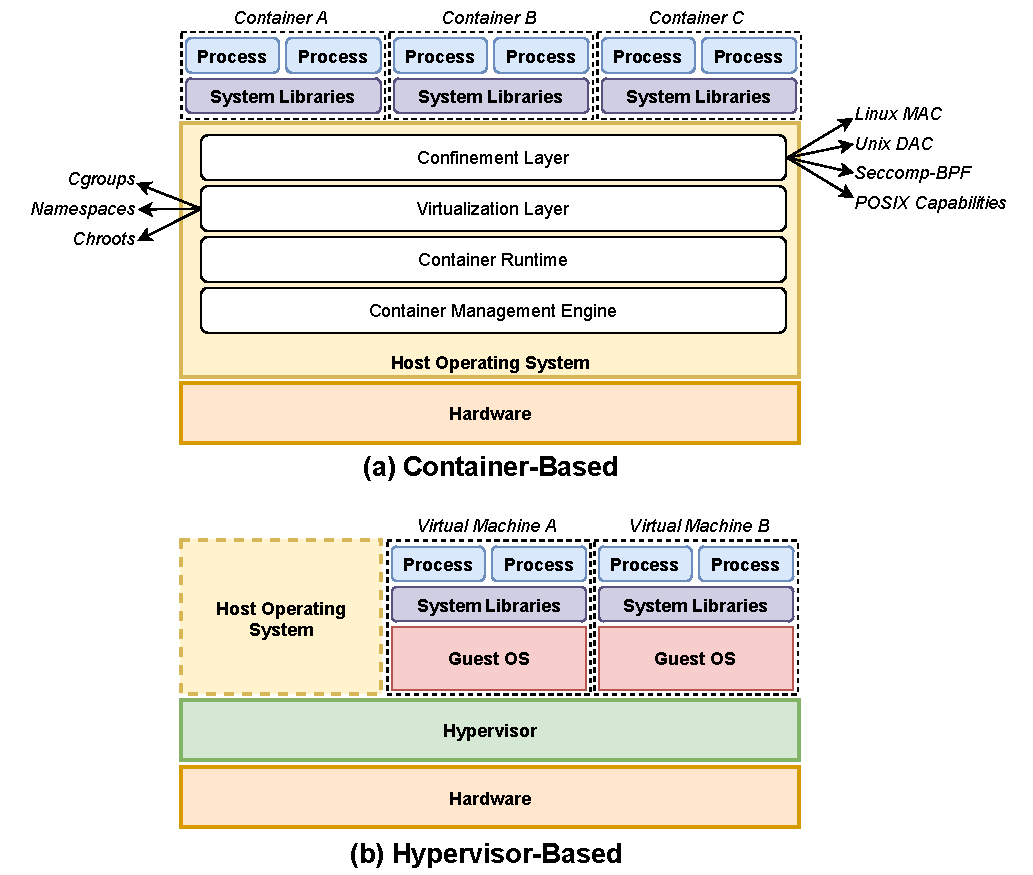
\includegraphics[width=0.8\linewidth]{figs/background/virtualization.pdf}
  \caption[A comparison of virtual machine and container architectures]{
    A comparison of virtual machine and container architectures. Containers \textbf{(a)}
    achieve virtualization using a thin layer provided by the host \gls{os}
    itself. They share the underlying operating system kernel and resources, requiring no
    guest \gls{os}. Type I hypervisors \textbf{(b)} virtualize and control the
    underlying hardware directly, but require full guest operating systems on top of the
    virtualization layer. Type II hypervisors \textbf{(c)} run on top of a host operating
    system but still require full guest operating systems above the virtualization layer.
  }%
  \label{fig:virt}
\end{figure}

\subsection{Container Security}%
\label{ss:container-security-bg}







\section{Extended BPF}%
\label{s:ebpf-bg}

\gls{ebpf} stands for \enquote{Extended \gls{bpf}}, though in reality it has very
little to do with Berkeley, packets, or filtering in its current
form~\cite{gregg2019_bpf}. In a nutshell, \gls{ebpf} is a Linux kernel technology that supports
dynamic system monitoring through the attachment of special \enquote{hooks} called \gls{bpf}
programs to specific kernel interfaces and userspace functions. In recent years, \gls{ebpf}'s
role has expanded, providing an interface to make extensions to the kernel as well as the
classic monitoring use case. In this section, we discuss the origins of \gls{ebpf}, its
components and how they work, its applications under the Linux kernel, and how it has
evolved over time.

\todo{Perhaps add a subsection here to discuss DTrace as a precursor to eBPF?}

\subsection{Origins of BPF\@: Efficient Packet Filtering and Beyond}%
\label{ss:origins-of-bpf-bg}

The original Berkeley Packet Filter, hereafter referred to as \gls{cbpf}\footnote{%
Throughout the rest of this thesis, we refer to extended \gls{bpf} using the terms
\enquote{\gls{ebpf}} and \enquote{\gls{bpf}} interchangeably. This is a matter of established
convention within the \gls{ebpf} community. Classic \gls{bpf} will be explicitly referred to by its
full name or the \gls{cbpf} acronym.}, arose out of a need to implement a more efficient packet
filtering mechanism for BSD Unix.  McCanne and Jacobson~\cite{mccanne1993_bpf} published
their work on \gls{cbpf} in 1993, marking an improvement over existing mechanisms in a number of
ways. Many of the reasons why classic \gls{bpf} was such an improvement over the status quo are
still relevant when discussing \textit{\gls{ebpf}}, and so we will briefly cover them here as
well.

In essence, classic \gls{bpf} is a \textit{register virtual machine} designed to take packets as
input and produce \textit{filtering decisions} as output. These filtering decisions could
then used to make decisions about whether a packet should be passed down to a more complex
pipeline for further analysis. The key insight behind \gls{cbpf} is that these filtering
decisions could be made more efficiently in \textit{kernelspace}, the part of the
operating system that runs in protection ring 0\footnote{Code that runs in ring 0 is said
to run with \textit{supervisor privileges} and is able to access all system memory. Ring
0 is the highest level of memory protection provided by the CPU~\cite{jaeger2008_os_security}.}
and which is most commonly associated with any parts of the operating system that do not
run in \textit{userland} (i.e.~the context of an ordinary user process). This provides
a considerable performance advantage over conventional approaches to network monitoring.
A typical network monitor runs in \textit{userspace}, meaning that packets need to be
copied over from kernelspace before they can be properly analyzed. This is an expensive
operation, requiring several context switches and potentially sleeping in the event of
a page fault~\cite{mccanne1993_bpf}.  By applying filtering logic in the kernel, this
expensive copying could be skipped for packets that would be discarded or ignored by the
network monitor anyway.

\begin{figure}[tbp]
  \centering
  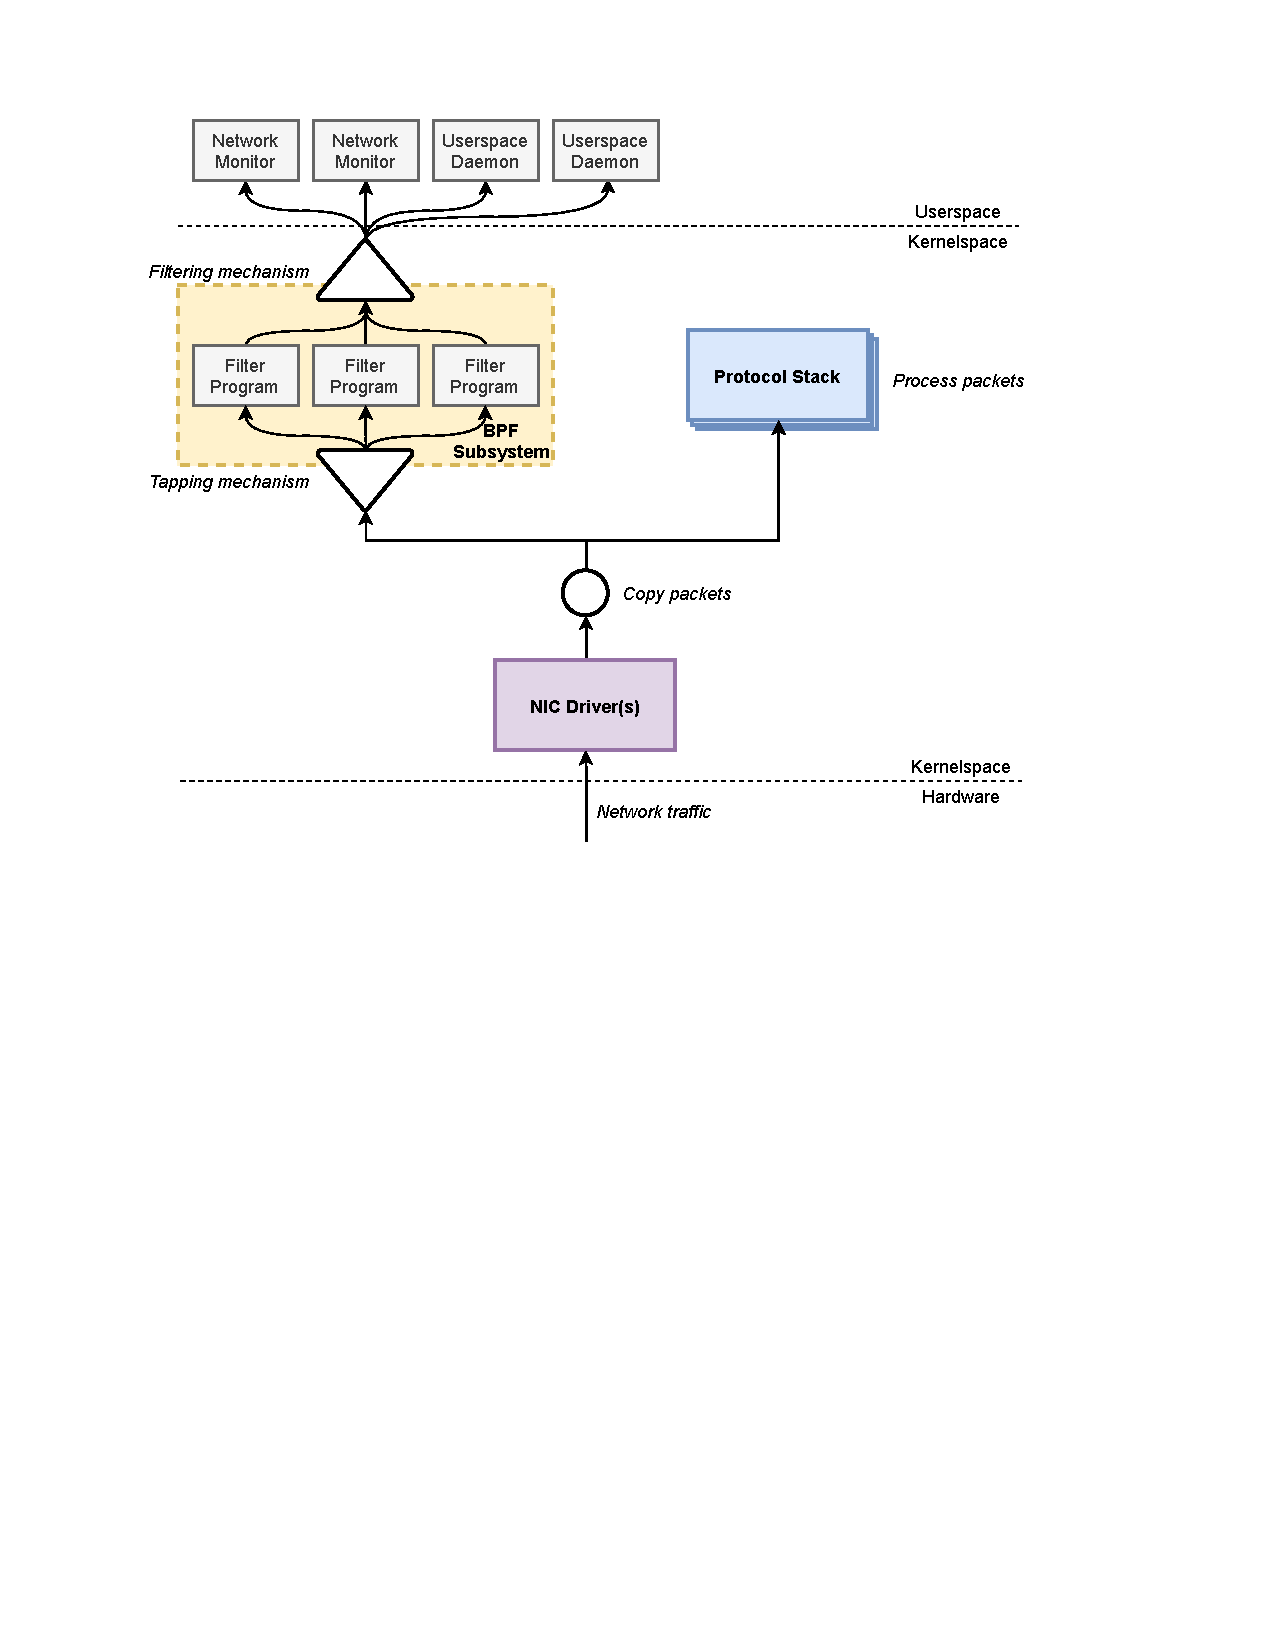
\includegraphics[width=0.8\linewidth]{figs/background/classic-bpf.pdf}
  \caption[The classic BPF architecture]{The classic \gls{bpf} architecture. Adapted from McCanne and Jacobson~\cite{mccanne1993_bpf}.}%
  \label{fig:classic-bpf}
\end{figure}

Classic \gls{bpf} can be divided into two major components: a \textit{tap} mechanism and a set
of one or more \textit{filter} programs. The cBPF architecture is depicted in
\Cref{fig:classic-bpf}. \gls{cbpf} programs are expressed as a control-flow graph (CFG)
over a set of abstract registers, backed by physical registers on the CPU. The tap
mechanism hooks into packets as they enter the networking stack, copying and forwarding
them to the filters. At runtime, the filter programs walk their control-flow graph, taking
the forwarded packets as input. As output, they return a filtering decision which controls
whether or not the packet should be forwarded to userspace~\cite{mccanne1993_bpf}.

Since its original introduction in 1993, classic \gls{bpf} has since been ported to a number of
Unix-like operating systems, including Linux~\cite{linux_bpf}, OpenBSD~\cite{openbsd_bpf},
and FreeBSD~\cite{freebsd_bpf}. Classic \gls{bpf} forms the backbone of widely used traffic
monitoring tools, most notably tcpdump~\cite{tcpdump, mccanne1993_bpf}. In Linux, the
\texttt{seccomp(2)} system call~\todo{CITE Anderson} was enhanced to include classic \gls{bpf}
filters, allowing a user process to use classic \gls{bpf} programs to define allowlists and
denylists of system calls (c.f.~\Cref{sss:seccomp}).

In 2014, Alexei Starovoitov and Daniel Borkmann~\cite{starovoitov2014_ebpf} first proposed
a total overhaul of the Linux \gls{bpf} engine. Their proposal, dubbed \gls{ebpf}, expanded the
classic \gls{bpf} execution model into a full-fledged virtual instruction set. In particular,
the extensions included a 512 byte stack, 11 registers (10 of which are general-purpose),
the ability to call a set of allowlisted kernel helper functions, the ability to attach
programs to a variety of system events, specialized data structures (called \gls{bpf} maps) to
store and share data at runtime, and an in-kernel verification engine to check for program
safety. At runtime, programs can be dynamically attached to system events and are
just-in-time compiled into the native instruction set.  \Cref{fig:extended-bpf} depicts
the \gls{ebpf} architecture in detail. The reader is encouraged to compare this with the classic
BPF architecture, depicted in \Cref{fig:classic-bpf}.

\begin{figure}[tbp]
  \centering
  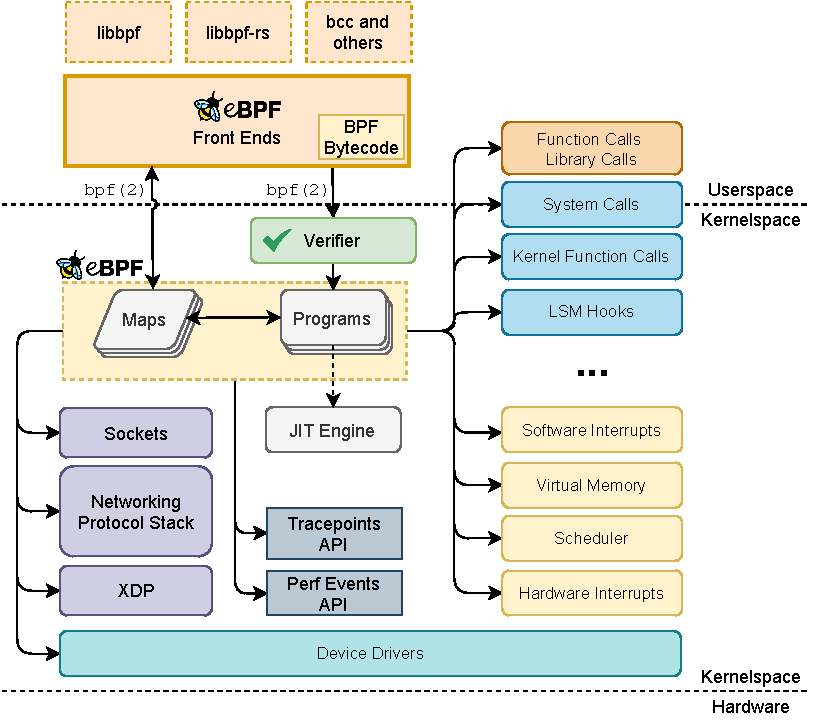
\includegraphics[width=0.8\linewidth]{figs/background/ebpf.pdf}
  \caption[The extended BPF architecture]{The extended \gls{bpf} architecture. Unlike classic
  \gls{bpf}, \gls{ebpf} programs are \gls{jit} compiled to the native instruction set, share data using
  specialized map data structures, and can be attached to many different kinds of system
  events. Programs can share data with each other and with the controlling userspace
  process using specialized map data structures. All \gls{ebpf} bytecode goes through
  a verification step before it can be loaded into the kernel.}%
  \label{fig:extended-bpf}
\end{figure}

While modern \gls{ebpf} has very little to do with the execution model of its older cousin, some
of the properties that made classic \gls{bpf} so performant still hold true today. In
particular, to notion of aggregating and processing data in kernelspace before
(optionally) handing it off to userspace is a key aspect of classic \gls{bpf} that has carried
over to \gls{ebpf}. What this means in practice is that \gls{ebpf} programs can be used to implement
very efficient monitoring software, harnessing the performance benefits of a pure
kernelspace implementation while maintaining the flexibility of a userspace
implementation.

\subsection{eBPF Programs}%
\label{ss:bpf-programs-bg}

\gls{ebpf} programs are expressed in a virtual RISC machine language called \gls{bpf} bytecode.  While
it is technically possible to write \gls{bpf} bytecode by hand, programs are most often compiled
from a restricted subset of the C programming language\footnote{Other languages may
eventually be used to write \gls{ebpf} programs as well.  For instance, an experimental \gls{ebpf}
target for the Rust programming language has recently been
proposed~\cite{decina2021_bpf_rust}. The important distinction here is that the set of all
possible \gls{ebpf} programs is a strict subset of the set of all possible programs.} using the
LLVM toolchain. Programs can be loaded and attached to system events using the
\texttt{bpf(2)} system call, at which point control passes to the \gls{ebpf} verifier, which
checks the programs to make sure they satisfy a set of safety
constraints~\cite{starovoitov2014_ebpf, gregg2019_bpf}. In particular, \gls{ebpf} programs must
consist of fewer than 1 million \gls{bpf} instructions and must not call into any kernel
functions outside of the allowlisted helpers. The program is also constrained to a 512
byte stack size; any additional memory required by the program must come from an \gls{ebpf} map
(c.f.~\Cref{ss:bpf-maps-bg}). For safety, memory accesses into allocated buffers must be
properly bounds checked, pointers must be null-checked before dereferencing, and any
access to external memory (e.g.~belonging to userspace programs or to the kernel itself)
must be read-only. Since \gls{ebpf} programs must provably terminate, no back-edges are
permitted in their control flow and all loops must be bounded by some fixed constant $i$
iterations.

To guard against data races, \gls{ebpf} programs always hold the kernel's RCU (read-copy-update)
lock while executing, gated by the \texttt{bpf\_prog\_enter} and \texttt{bpf\_prog\_exit}
functions in the kernel. In simple terms, the RCU lock allows concurrent reads, except in
the presence of updates, optimizing for read-mostly workloads (i.e.~precisely the sort of
workload \gls{ebpf} is designed for)~\cite{mckenney2007_rcu}. This implicitly enables \gls{bpf}
programs to read from many common kernel data structures without fear of data races and
simultaneously protects reads and updates to \gls{ebpf} maps, at a slight (albeit reasonable)
performance penalty~\cite{mckenney2007_rcu}. In addition to holding the RCU lock, \gls{ebpf}
programs are not considered \textit{preemptable} by default. In practice, this means that
\gls{ebpf} programs cannot sleep and must run to termination on their assigned core. This
property, while useful in many circumstances, enforces undesirable limitations on \gls{ebpf}
helpers, since it precludes any functionality that may cause the program to sleep (e.g.~a
page fault). To account for use cases where sleeping is unavoidable, Linux 5.10 introduced
sleepable versions of some \gls{ebpf} program types~\cite{starovoitov2020_sleepable}.

Once loaded into the kernel, \gls{ebpf} programs are represented as \gls{bpf} objects, each with its
own reference count. Loading a \gls{bpf} program and attaching it to a system event increments
the reference count, while detaching and unloading the program decrements the reference
count. The kernel also exposes a special filesystem, \gls{bpffs}, which allows \gls{bpf}
programs to be pinned. This also increments the reference count, allowing an attached
program to outlive its controlling process (i.e.~the process that loaded and attached
it)~\cite{gregg2019_bpf}.

\subsubsection*{Working with the Verifier}

In practice, the restrictions imposed by the verifier mean that \gls{ebpf} programs are not
\textit{Turing-complete}~\cite{gregg2019_bpf}.  This property is required, given that the
halting problem (i.e.~the decidability of program termination) is known not to be solvable
for Turing-complete programs. This notion of Turing-incompleteness means that the set of
all possible \gls{ebpf} programs is a strict subset of the set of all possible C programs. While
these limitations help to ensure program safety, they also naturally restrict some
operations which \textit{may} be safe but are not strictly verifiable. To overcome the
limitations imposed by the verifier and achieve this safe-yet-unverifiable behaviour, \gls{ebpf}
programmers have a few tools in their arsenal. For instance, a specific set of allowlisted
kernel helpers offers the ability to call into specific kernel functions, bypassing the
limitations imposed by the \gls{ebpf} verifier. As a simple example, the
\texttt{bpf\_probe\_write\_user()} helper allows an \gls{ebpf} program to write to a userspace
memory address, bypassing the read-only restrictions imposed by the verifier. While these
allowlisted helpers operate in a \textit{mostly} unrestricted context, their usage
\textit{is} restricted at the function call boundary, ensuring that the \gls{ebpf} program obeys
the safety contract specified by the helper function.  Another common design pattern is
using a dummy \gls{ebpf} map as a scratch buffer to reserve a larger amount of memory for the
\gls{ebpf} program.  Since \gls{ebpf} programs cannot sleep~\cite{gregg2019_bpf}, dynamic memory
allocation within the \gls{bpf} context is impossible. These dummy maps offer a way to access
additional memory from a pool reserved at the time the map was loaded into the kernel.

\subsubsection*{eBPF Program Types and Use Cases}

Each \gls{ebpf} program has a specific \textit{program type}, which determines both the set of
system events to which the program can attach and the set of allowed kernel helpers that
can be called from within the program context. Each program type roughly corresponds with
a distinct \gls{ebpf} use case. For the purposes of this thesis, we will primarily be dealing
with \textit{\gls{lsm} probes}, \textit{raw tracepoints}, \textit{fentry/fexit probes}, and
\textit{uprobes/uretprobes}, as they form the basis of \bpfbox{} and \bpfcontain{}'s
kernelspace implementations. \Cref{tab:program-types} summarizes the relevant program types
and their properties.

\begingroup\footnotesize
\begin{longtable}[c]{lp{4.2in}}
\caption[A selection of relevant eBPF program types for \bpfbox{} and \bpfcontain{}]{A selection of relevant \gls{ebpf} program types for \bpfbox{} and \bpfcontain{}.}%
\label{tab:program-types}\\
  \toprule
  Program Type & Description\\
  \midrule
  \textit{\gls{lsm} Probes}    & \gls{lsm} probes~\cite{singh2019_krsi} attach to the kernel's \gls{lsm} hooks and can be used to audit security events and make policy decisions.\\
  \textit{Raw Tracepoints}     & Raw tracepoint programs attach to a stable tracing interface exposed by the Linux kernel. Tracepoints are considered a stable API, but are more limiting than alternatives such as Kprobes or Fentry probes.\\
  \textit{Kprobes/Kretprobes}  & Kprobe programs can attach to any kernel function, by replacing the function with a trap into the \gls{bpf} program. The \gls{bpf} program has read-only access to the function arguments. Kretprobes work in the same way, but handle function returns instead of function calls.\\
  \textit{Fentry/Fexit Probes} & A more efficient version of Kprobes and Kretprobes that directly trampolines into the \gls{bpf} program instead of trapping. These programs can also be used to modify the return value of specifically allowlisted kernel functions (e.g.~system call implementations).\\
  \textit{Uprobes/Uretprobes}  & The userspace equivalent of Kprobes and Kretprobes.\\
  \bottomrule
\end{longtable}
\endgroup

\subsubsection*{LSM Probes: Making Security Decisions with eBPF}

It is worth spending more time focusing specifically on \gls{lsm} probes, as these are used
extensively in \bpfbox{} and \bpfcontain{} to enforce policy over security-sensitive
events. Introduced by KP Singh in his KRSI (Kernel Runtime Security Instrumentation)
patch~\cite{singh2019_krsi}, \gls{lsm} probes define a canonical framework for attaching \gls{ebpf}
programs to the Linux kernel's \gls{lsm} security hooks (c.f.~\Cref{ss:mac}). Unlike
traditional \gls{lsm}s which are implemented as static kernel modules, \gls{lsm} probes are
\textit{dynamically attachable}, meaning that \gls{mac} and audit policy can be adjusted at
runtime, simply by loading a new \gls{ebpf} program.  \Cref{fig:bpf-lsm} depicts how \gls{lsm} probes
integrate with the \gls{lsm} framework.

\begin{figure}[tbp]
  \centering
  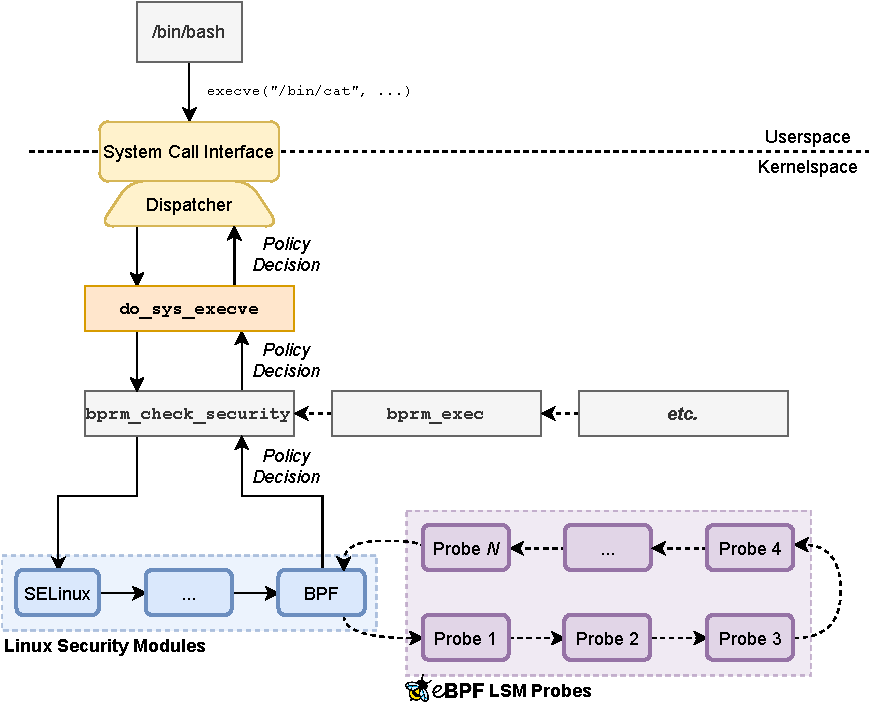
\includegraphics[width=0.8\linewidth]{figs/background/bpf-lsm.pdf}
  \caption[How eBPF LSM probes make policy decisions]{A simplified example of how \gls{ebpf} \gls{lsm} probes make policy decisions. Privileged userspace processes can attach one or more \gls{lsm} probes to a given hook. When a userspace process requests a privileged operation, the kernel implicitly calls into the corresponding \gls{lsm} hooks, which in turn invoke the logic associated with each \gls{lsm}. A shim \gls{lsm} is responsible for invoking each \gls{lsm} probe, and any resulting policy decisions are taken together to arrive at a final decision. As with ordinary \gls{lsm}s, the final decision is consensus-based. That is, if \textit{any \gls{lsm}s} or \textit{any \gls{bpf} \gls{lsm} probes} disagree on a policy decision, the privileged operation is denied.}%
  \label{fig:bpf-lsm}
\end{figure}

As with other LSMs, LSM probes implement a form of mandatory access control. Each LSM
probe can be attached to one or more LSM hooks defined in the kernel. When the hook fires
(i.e.~when a task requests a privileged operation form the kernel), every attached probe
fires as part of the normal LSM pipeline. The body of the \gls{bpf} program defines filtering
and audit logic, optionally accessing maps to store and query persistent state. The \gls{bpf}
program then returns a security decision about whether the requested operation should be
allowed or denied.  In order for an operation to be allowed, \textit{all} other LSMs and
LSM probes must agree on the policy decision and ordinary security checks performed by the
operating system must also succeed. In other words, it is not possible to grant additional
privileges using an LSM probe.

Owing to the properties discussed earlier in this section, \gls{ebpf} confers a natural
flexibility to LSM probes quite unlike that of traditional LSM-based security frameworks.
In particular, LSM probes can be attached at runtime and can cooperate with other \gls{ebpf}
program types using \gls{ebpf} maps (c.f.~\Cref{ss:bpf-maps-bg}). This notion of cooperating
programs presents an opportunity to design modular policy enforcement mechanisms that
operate beyond the scope of the LSM hooks framework itself.  Another key advantage of LSM
probes over traditional LSMs lies in their adoptability.  While industry actors may be
understandably reluctant to adopt \enquote{yet another out-of-tree LSM}, a security
mechanism based on \gls{ebpf} does not carry the same technical baggage.  \gls{ebpf} programs are safe
to use in production and can be deployed at runtime on an unmodified kernel.  This makes
\gls{ebpf} a particularly attractive target for developing new security solutions.

\subsection{eBPF Maps}%
\label{ss:bpf-maps-bg}

\gls{ebpf} maps serve as both a runtime data store for \gls{ebpf} programs and the canonical method of
communication between \gls{ebpf} programs and other \gls{ebpf} programs, and \gls{ebpf} programs and
userspace applications. Like \gls{ebpf} programs, maps can be pinned to \gls{bpffs} to
increment their reference count in the kernel. Concurrent access to \gls{ebpf} maps from within
kernelspace is protected by an implicit RCU lock, and a spinlock concurrency primitive is
exposed via a helper function to guard map accesses between kernelspace and userspace.
From the \gls{ebpf} side, maps can be accessed using a set of provided helper functions.
Userspace applications can access maps using the \texttt{bpf(2)} system call or through
direct memory-mapping (only available for arrays) via
\texttt{mmap(2)~\cite{gregg2019_bpf}}. While many \gls{ebpf} maps are designed to be generic,
others are highly specialized for specific use cases. \bpfcontain{} and \bpfbox{} make
use of several \gls{ebpf} map types, which are summarized in \Cref{tab:map-types}.

\begingroup\footnotesize
\begin{longtable}[c]{lp{3.9in}}
\caption[A selection of relevant eBPF map types for \bpfbox{} and \bpfcontain{}]{A selection of relevant \gls{ebpf} map types for \bpfbox{} and \bpfcontain{}.}%
\label{tab:map-types}\\
  \toprule
  Map Type & Description\\
  \midrule
  \textit{\gls{bpf} Hashmap}           & A key-value hashmap. Keys and values can be arbitrary data structures.\\
  \textit{\gls{bpf} Array}             & A fixed-size array with integer indices. Values can be arbitrary data structures.\\
  \textit{\gls{bpf} Array/Map of Maps} & A \gls{bpf} array or map that stores handles into \textit{other maps}.\\
  \textit{\gls{bpf} Per-CPU Array/Map} & Like a \gls{bpf} hashmap or \gls{bpf} array but with a separate copy per logical CPU\@. This enables concurrent access across CPUs, but without synchronization.\\
  \textit{\gls{bpf} Local Storage}     & A dummy \gls{bpf} map that provides a handle into local storage for a given kernel data structure. For instance, task local storage provides storage per-task-struct. Values can be arbitrary data structures.\\
  \textit{\gls{bpf} Ringbuf}           & A concurrent circular buffer that passes event handles from kernelspace to userspace. To communicate, \gls{ebpf} programs submit events and userspace applications poll events.\\
  \bottomrule
\end{longtable}
\endgroup

\subsection{Userspace Front-Ends}%
\label{ss:bpf-userspace}

Although \gls{ebpf} programs and maps can exist on their own after being pinned to
\gls{bpffs}, the more common approach is to manage their lifetime using a controlling
process. Userspace applications implementing such a controlling process typically use an
\gls{ebpf} front-end framework to facilitate loading and interacting with programs and maps.
A number of such front-ends exist~\cite{gobpf, bcc, libbpf, libbpf-rs, libbpfgo,
cilium-ebpf, redbpf}, some more practical than others.
\textit{bcc}~\cite{bcc} was the first \gls{ebpf} framework to offer high-level userspace tooling
around \gls{ebpf}, providing an LLVM backend for compiling \gls{ebpf} programs and a Python library
for loading and interacting with them. \textit{libbpf}~\cite{libbpf} offers a pure
C alternative to bcc and has since been upstreamed into the Linux kernel.
\textit{libbpf-rs}~\cite{libbpf-rs} and \textit{libbpfgo}~\cite{libbpfgo} offer Rust
and Golang bindings for libbpf respectively. Other tooling~\cite{cilium-ebpf, redbpf}
bypasses libbpf entirely, providing fully native \gls{ebpf} bindings for Rust and Golang.

\subsubsection*{Libbpf and BPF CO-RE}%

Among the myriad of userspace front-ends available for \gls{ebpf}, libbpf stands out as the only
one with official upstream support from the Linux kernel. Recent improvements to libbpf
have solidified its position as the dominant framework. In particular, libbpf supports
a new way of compiling a loading \gls{bpf} programs into the kernel, \gls{bpf}
\gls{core}~\cite{gregg2020_core, nakryiko2020_core}. \gls{bpf} \gls{core} uses \gls{btf}
debugging information exposed by the kernel, along with load-time relocation logic to
support loading the same compiled \gls{ebpf} bytecode across multiple target kernels. The
precise technical details of how \gls{core} works are beyond the scope of this thesis.

With libbpf and \gls{core}, \gls{ebpf} programs can now be compiled once and run on any target kernel
that supports the required \gls{bpf} features. This provides a powerful advantage over other
\gls{ebpf} frameworks and even alternatives to \gls{ebpf}, such as loadable kernel modules. A \gls{core}
program that runs on one kernel will be guaranteed to run on another of the same version
or higher, barring any API incompatibilities like changes in a hooker function signature.
Such incompatibilities can be resolved with the use of built-in kernel configuration
checks.

\bpfcontain{} (c.f.~\Cref{c:bpfcontain}) leverages libbpf and \gls{core} through libbpf-rs, the
canonical Rust bindings for libbpf, providing adoptability advantages over the original
\bpfbox{} prototype (c.f.~\Cref{c:bpfbox}), which uses bcc.

\subsection{Comparing eBPF with Loadable Kernel Modules}%
\label{ss:bpf-vs-modules}

Before \gls{ebpf}, the primary means of modifying the Linux kernel at runtime was through the
use of \textit{loadable kernel modules}~\cite{corbet1998_device_drivers}. A kernel module
can be thought of as a discrete bundle of code that can be loaded into the kernel (or
compiled into its binary image). Like other kernel code, including \gls{ebpf}, modules are
event-based and run in ring 0, responding to and handling system events as they occur.
Since kernel modules and \gls{ebpf} can serve similar (but not strictly equivalent) purposes,
comparing the two can offer some insight about how they differ and which technology is
better fit for a specific purpose.

At a first approximation, \gls{ebpf} differs from kernel modules in the following meaningful ways~\cite{gregg2019_bpf}:
\begin{enumerate}
  \item \gls{ebpf} programs \textbf{must pass verification checks} before they can be loaded into the
  kernel. This verification step provides assurances about program safety. For instance, \gls{ebpf}
  programs are guaranteed not to deadlock the kernel, and are far less likely to suffer from
  memory safety issues. In contrast, misuse of kernel APIs in a kernel module can have dangerous
  implications for system safety and security.

  \item An implicit advantage provided by \gls{ebpf} is that \gls{bpf} programs can be \textbf{easier
  to reason about} than other kernel code. \gls{ebpf} abstracts away much of the complex
  functionality required to make kernel code operate correctly by providing implicit
  guarantees about program execution. Even helper functions, which offer functionality
  beyond the scope of verifiability, must obey a predetermined contract with the verifier
  in order to be considered safe. Thus, when an \gls{ebpf} program passes verification, there is
  a much higher likelihood that it will \enquote{just work.}

  \item \gls{ebpf} \textbf{exposes map-like data structures} to facilitate runtime data storage,
  communication between \gls{ebpf} programs, and communication with userspace applications. In
  the case of kernel modules, data structures often must be implemented by hand, taking
  great care not to introduce potential bugs or security vulnerabilities, particularly in
  the case of memory management. Communication with userspace from a kernel module might
  be done via netlink sockets, file operations, or similar
  means~\cite{corbet1998_device_drivers}. These modes of communication are often less
  streamlined and, in the case of file operations, must be implemented by hand, increasing
  the likelihood of programmer error.

  \item \gls{ebpf} programs are \textbf{not Turing-complete}. Intuitively, this means that
  the set of operations a kernel module can perform is a strict superset of \gls{ebpf}. While
  this may appear to be a hugely limiting factor, in practice \gls{ebpf} programs are often
  sufficient to implement sophisticated tracing, filtering, and policy enforcement logic.
  Where the verifier gets in the way, the programmer can reach for a number of helper
  functions provided by the kernel to achieve more complex behaviour.

  \item \gls{ebpf} is \textbf{not suitable for implementing device drivers} or other complex
  functionality that requires ad-hoc access to various kernel facilities and write access
  to arbitrary memory locations.
\end{enumerate}

In summary, \gls{ebpf} is useful for observability use cases, or cases in which the functional
requirements of the kernel code are not expected to be complex or might be expected to
change frequently. \gls{ebpf} programs and maps are particularly good at separation of concerns,
composability, and modularity. \gls{ebpf} maps facilitate easy communication between kernelspace
and userspace, and provide the ability to build relationships between data from different
program types. Kernel modules should be preferred for the implementation of more complex
kernel functionality, such as device drivers.
